\chapter{Methods and Materials}
\section{Wastewater treatment plant description}
\subsection{Process and data sources in SWHEPP}
Shek Wu Hui Effluent Polish Plant (SWHEPP) is a secondary sewage treatment plant, which treats the municipal wastewater of the Sheung Shui, Fanling Districts and adjacent areas, and treated leachate effluent from North East New Territories (NENT) leachate treatment plant. The plant is designed for 300,000 population equivalents (PE) in 2001, and in 2009, the daily treatment capacity has been expanded from 80,000 m$^3$/day to 93,000 m$^3$/day. SHWEPP is operated and maintained by Drainage Services Department (DSD), and the plant will be upgraded to teritary treatment level to increase the treatment capacity of 190,000 m$^3$/day by the end of 2025. As shown in Fig.~\ref{fig:SHWEPP-flowchart}, the treatment plant is mainly comprised of primary sedimentation, secondary biological treatment, and final sedimentation followed by a membrane bioreactor (MBR), which provides an advanced level of organic and suspended solids removal. To monitor the effluent quality at real-time, low volume of the MBR effluent is pumped to a sampling tank near by the MBR location. Two on-line meters, ammoniacal nitrogen on-line sensor and colour level on-line analyzer are installed in the sampling tank, which are indicated as (a) and (b) in Fig.~\ref{fig:SHWEPP-flowchart}.

\begin{figure}[h]
    \centering
    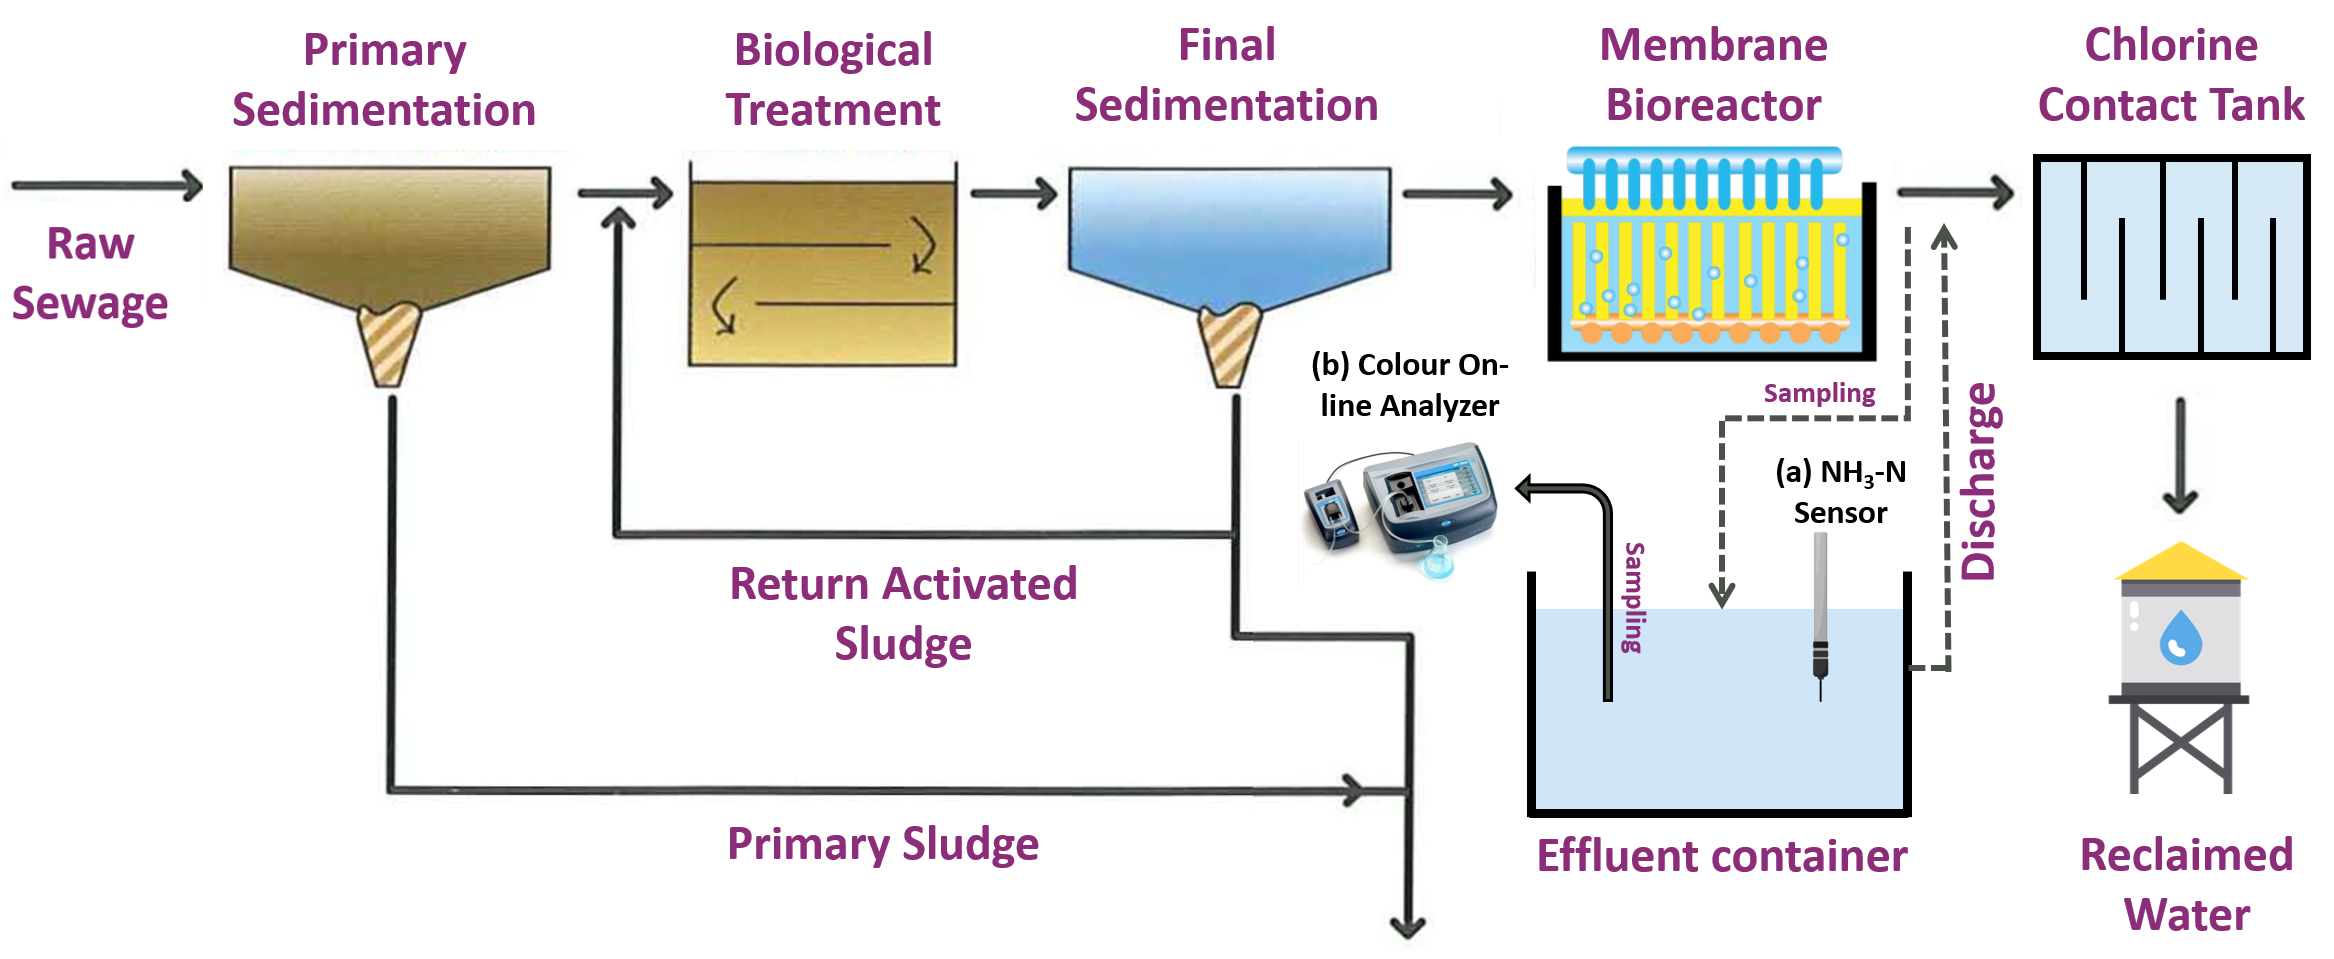
\includegraphics[width=0.9\columnwidth]{imgs/Sewage-treatment-process-flowchart.png}
    \caption{Sewage treatment process flowchart at SWHEPP (adapted from Drainage Services Department 2020)}
    \label{fig:SHWEPP-flowchart}
\end{figure}

\subsection{Reclaimed water standard}
Reclaimed water for non-potable reuses can serve for irrigation for agricultures, toilet flushing and irrigation for landscaping, etc. Water Supply Department (WSD) will soon implement a reclaimed water supply system in SWHEPP by disinfecting the teriary treated sewage (i.e., MBR permeate). The produced reclaimed water will be served for non-potable reuses and is required to satisfy the water quality standards, shown in Table.~\ref{tab:reclaimed-standard}.

\begin{table}[!ht]
    \centering
    \caption{\label{tab:reclaimed-standard}Endorsed Reclaimed Water Quality Standards from Water Supply Department.}
    \begin{NiceTabular}{lcl}
        \toprule
        Parameter & Unit & Requirement \tabularnote{The water quality standards for all parameters are applicable at the point-of-use of the system.} \\
        \midrule
        \textit{E. coli} & cfu/100 mL & Not detectable \\ 
        Colour & Hazen Unit & $\le$ 20 \\ 
        Ammoniacal Nitrogen (NH$_3$-N) & mg/L as N & $\le$ 1 \\ 
        Total Residual Chlorine & mg/L & $\ge$ 0.2 \\ 
        Dissolved Oxygen & mg/L & $\ge$ 0.2 \\ 
        Turbidity & NTU & $\le$ 5 \\ 
        5-day Biochemical Oxygen Demand & mg/L & $\le$ 1 \\ 
        pH & - & 6-9 \\ 
        Threshold Odour Number & - & $\le$ 100 \\ 
        Synthetic detergents & mg/L & $\le$ 5 \\
        \bottomrule
    \end{NiceTabular}
\end{table}

\section{Data collection and preparation}
\subsection{Ammonia data monitoring and collection}
Ammonium and Potassium Probe for IQ Sensor Net System
The WTW ISE sensor AmmoLyt®Plus 700 IQ is a rugged, ion selective electrode (ISE) probe for the IQ Sensor Net process monitoring system. The AmmoLyt provides continuous and reagentless monitoring of ammonium and potassium using the most precise and reliable electrodes on the market. The individually replaceable electrodes have a typical lifetime of 18 to 24 months and are warrantied for 1 year minimizing maintenance effort and ownership cost.  
\subsection{Color data monitoring and collection}

\subsection{Metrics for model evaluation}

AI methods have been demonstrated to be effective in controlling chlorination, while ML models are effective in modeling DBP concentrations, as well as modeling important parameters for adsorption and membrane-filtration processes. The results are often evaluated using various statistical measures including the coefficient of correlation (R), the coefficient of determination (R2), the mean average error (MAE), the mean square error (MSE), the root mean square error (RMSE), and relative error (RE).
\subsection{Data cleaning and pre-processing}

The original data were embedded in multiple matrices and were very messy, with missing values, bad data cells, and unnecessary information. Therefore, the Python modules Numpy (Oliphant, 2006) and Pandas (McKinney, 2010) were used to prepare an organized ‘clean’ dataset for analysis. This dataset contained 105,861 samples (data points) with 34 variables, giving a matrix size of 105,861 × 34. The samples were organized in time series with 10min intervals. 

However, the raw high-resolution data from each meter were compressed by averaging over 10-minute periods to obtain time series with temporal resolutions of 10 min.

Most AI techniques were modeled using experimental data to simulate, predict confirm, and optimize contaminant removal in wastewater treatment processes. Experimental data set were either divided into three parts (training, validation, and testing) or two parts (training and testing). The training set was used to develop the model, the validation data set was used to optimize the model, and the testing data set was used to test the model in the prediction stage.

\subsubsection{Data smoothing with Savitzky-Golay filter}
\subsubsection{Exponentially Weighted Moving Average}
\subsubsection{Outlier Removal}

\subsection{Data transformation}
Split of Train/valid/test dataset 
\section{Architecture design of the selected baseline models}
\subsection{Random Forest}
F can be described as an ensemble method in which the final result is obtained by aggregating (through averaging in the case of regression) results from multiple weak learners known as Classification and Regression Trees (CARTs) (Breiman, 2017). Each weak learner (tree) is trained on the bootstrap set, which is obtained by sampling with replacement from the original training set. For trees, the input variables are used to generate nodes. These variables are selected partially and randomly as a subset in every split, then the variable contributing to the smallest sum of impurity of two child nodes at a certain split point is chosen as the split variable. This is done repeatedly until the trees don't need to split anymore. The regression impurity of a particular node is defined by Eqs. (2), (3) and (4), \citep{wangMachineLearningFramework2021}
\subsection{LSTM}
Recently, deep recurrent neural networks (RNN) such as long short-term memory networks (LSTM) have shown breakthrough results over state-of-the-art machinelearning methods in many applications with non-linear temporal data, including robotics, high-energy physics and computational geometry (Goodfellow et al. 2016). These methods can successfully engineer appropriate long-term temporal dependencies and variable length features, significantly lessening the need to pre-process data with respect to traditional machine-learning methods or statistical approaches. It is the ability to capture the long-term dependencies that make LSTM networks particularity fitting for the problem at hand. 

Fig. 1 The general schema of a RNN unit versus a LSTM one (adapted from Olah 2015)

Architecture of the method proposed by Mamandipoor et al. (2020)

\subsection{RNN}

\subsection{GRU}

\section{Implementation of regularization}

\subsection{Scheduler}

